\documentclass[11pt]{article}

\usepackage[review]{acl}

\usepackage{times}
\usepackage{latexsym}
\usepackage[T1]{fontenc}
\usepackage[utf8]{inputenc}
\usepackage{microtype}
\usepackage{inconsolata}
\usepackage{graphicx}

\usepackage{amsmath,amssymb}
\usepackage{booktabs}
\usepackage{multirow}
\usepackage{xcolor}
\usepackage{tikz}
\usetikzlibrary{arrows.meta,positioning,calc,shapes.geometric,decorations.pathreplacing}
\usepackage{pgfplots}
\pgfplotsset{compat=1.18}
\usepgfplotslibrary{groupplots}

% ---------- palette ----------
\definecolor{interface}{HTML}{E8730C}
\definecolor{decoder}{HTML}{3C78B4}
\definecolor{derivative}{HTML}{C0392B}
\definecolor{benign}{HTML}{4C9A5B}
\definecolor{moderate}{HTML}{E1A93A}
\definecolor{severe}{HTML}{C0392B}
\definecolor{featlow}{HTML}{A9CBEA}
\definecolor{featmid}{HTML}{5B8DC9}
\definecolor{feathigh}{HTML}{2E5A9C}

\DeclareRobustCommand*\circled[1]{\tikz[baseline=(char.base)]{\node[shape=circle,draw,inner sep=0.8pt,font=\scriptsize\bfseries] (char) {#1};}}
\newcommand{\Tp}{\mathcal{T}'}
\newcommand{\refit}{ReFit}
\newcommand{\refitI}{ReFit-interface}
\newcommand{\refitF}{ReFit-full}
\newcommand{\ci}[2]{\,[#1,\,#2]}

\title{ReFit: Repairing Speculative Drafters\\for Post-Trained Language Models}

\author{Anonymous ACL submission}

\begin{document}
\maketitle

\begin{abstract}
Speculative decoding with target-conditioned drafters such as EAGLE-3 is among the fastest ways to serve large language models, and the drafter released with a base model is routinely reused for its many post-trained derivatives.
We show that this reuse breaks for an important and growing class of models: derivatives shaped by extensive off-policy post-training, such as today's distilled reasoning models.
In a census of public derivatives, quantized, merged and on-policy RL models retain 96--103\% of the family drafter's acceptance, while extensively post-trained reasoning models lose up to 30\%, erasing most of the speedup.
Post-training shifts both the hidden states the drafter reads and the tokens it must predict, even on text the derivative did not write.
We introduce \emph{\refit{}}, which re-fits a family drafter on the derivative's own responses to public instructions, without any of the original training data.
Re-fitting the whole warm-started drafter closes 72\% of the gap to a dedicated drafter trained specifically for the derivative, and re-fitting only its \emph{feature interface}, the projection through which it reads the target (12\% of its parameters), closes 60\%, using 11 GPU-hours, two orders of magnitude less compute than the public recipe for a dedicated drafter.
On DeepSeek-R1-Distill-Llama-8B, \refit{} raises the end-to-end speedup from 1.31$\times$ to 1.83$\times$ on SPEED-Bench (dedicated drafter: 2.05$\times$) and from 1.48$\times$ to 2.31$\times$ on MATH-500, and on Llama-3.1-Nemotron-Nano-8B from 1.29$\times$ to 1.80$\times$; it outperforms independent draft models and carries over to a second model family, sampled decoding and reasoning traces thousands of tokens long.
\end{abstract}

% =====================================================================
\section{Introduction}
% =====================================================================

Speculative decoding has become the standard way to serve large language models (LLMs) quickly: a small drafter proposes several tokens, and the target model verifies all of them in a single forward pass, accelerating generation without changing its output \citep{leviathan2023speculative,chen2023accelerating}.
The fastest drafters today are \emph{target-conditioned}.
Rather than modeling text from scratch, they read the target's own hidden states and predict its next tokens from them \citep{cai2024medusa,li2024eagle,li2025eagle3,chen2026dflash}.
EAGLE-3, for instance, fuses features from the target's lower, middle and upper layers and reports speedups of up to 6.5$\times$ \citep{li2025eagle3}.
The price of this coupling is that each drafter is trained for one specific target, on hundreds of thousands of examples, for tens of epochs.

Open-weight models, however, rarely stay single models.
A popular base model such as Llama-3.1-8B spawns thousands of derivatives on public model hubs, from quantized and merged variants to RL-tuned checkpoints and reasoning distillations \citep{horwitz2025atlas}.
Training a dedicated drafter for each one is out of reach, so serving stacks reuse the drafter released for the family's instruction model, the \emph{family drafter}, for all of its relatives \citep{kwon2023vllm,redhat2025speculators}.
Two questions behind this practice remain open: when does a family drafter keep working for a derivative, and what can be done when it does not?

\begin{figure}[t]
  \centering
  % Figure 1: teaser. (a) every eligible derivative in the focused SPEED-Bench cohort; (b) speedup on R1-Distill.
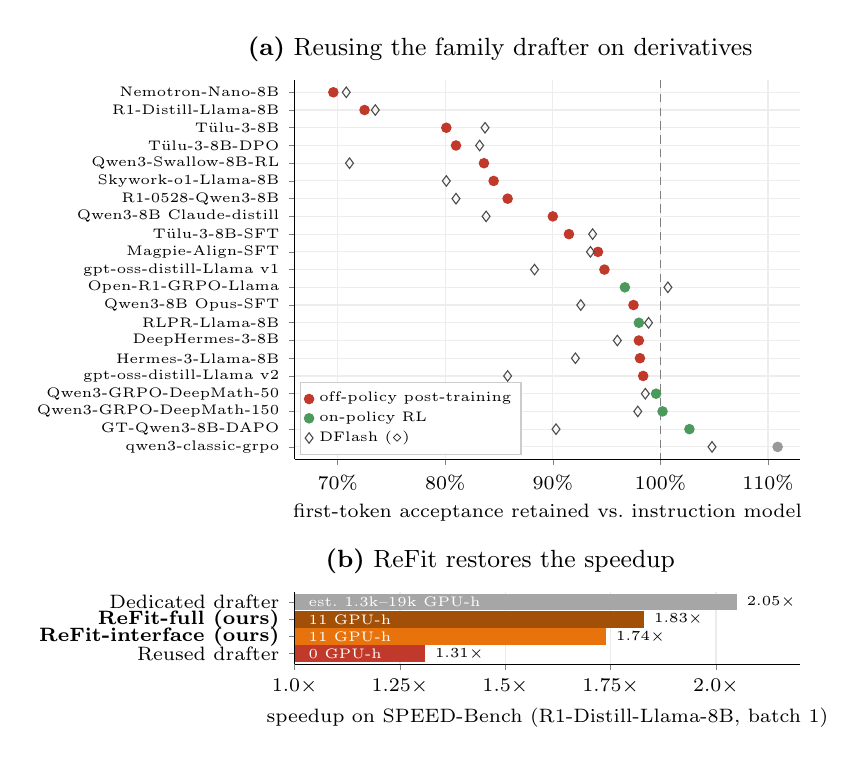
\begin{tikzpicture}
% ---------------- (a) focused cohort ----------------
\begin{axis}[name=census,
  width=0.66\columnwidth, height=6.4cm, scale only axis=false,
  xmin=0.66, xmax=1.13,
  ymin=0.3, ymax=21.7, y dir=reverse,
  ytick={1,...,21},
  yticklabels={Nemotron-Nano-8B,R1-Distill-Llama-8B,T\"ulu-3-8B,T\"ulu-3-8B-DPO,Qwen3-Swallow-8B-RL,Skywork-o1-Llama-8B,R1-0528-Qwen3-8B,Qwen3-8B Claude-distill,T\"ulu-3-8B-SFT,Magpie-Align-SFT,gpt-oss-distill-Llama v1,Open-R1-GRPO-Llama,Qwen3-8B Opus-SFT,RLPR-Llama-8B,DeepHermes-3-8B,Hermes-3-Llama-8B,gpt-oss-distill-Llama v2,Qwen3-GRPO-DeepMath-50,Qwen3-GRPO-DeepMath-150,GT-Qwen3-8B-DAPO,qwen3-classic-grpo},
  yticklabel style={font=\tiny},
  xticklabel style={font=\scriptsize},
  xtick={0.7,0.8,0.9,1.0,1.1},
  xticklabels={70\%,80\%,90\%,100\%,110\%},
  axis x line*=bottom, axis y line*=left,
  tick align=outside, major tick length=2pt,
  ymajorgrids, xmajorgrids, grid style={black!7},
  xlabel={\scriptsize first-token acceptance retained vs.\ instruction model},
  xlabel style={yshift=2pt},
  title={\small\textbf{(a)} Reusing the family drafter on derivatives},
  title style={yshift=-3pt, xshift=-6mm},
  legend style={font=\tiny, draw=black!20, fill=white, at={(0.01,0.01)}, anchor=south west, cells={anchor=west}, row sep=-2pt, inner sep=1.5pt},
  clip=false,
]
\draw[densely dashed, black!50] (axis cs:1.0,0.3) -- (axis cs:1.0,21.7);
% off-policy post-training (EAGLE-3)
\addplot[only marks, mark=*, mark size=1.7pt, color=severe] coordinates {
  (0.696,1) (0.725,2) (0.801,3) (0.810,4) (0.836,5) (0.845,6) (0.858,7) (0.900,8) (0.915,9) (0.942,10) (0.948,11)
  (0.975,13) (0.980,15) (0.981,16) (0.984,17)};
\addlegendentry{off-policy post-training}
% on-policy RL (EAGLE-3)
\addplot[only marks, mark=*, mark size=1.7pt, color=benign] coordinates {
  (0.967,12) (0.980,14) (0.996,18) (1.002,19) (1.027,20)};
\addlegendentry{on-policy RL}
% undocumented history
\addplot[only marks, mark=*, mark size=1.7pt, color=black!40, forget plot] coordinates {(1.109,21)};
% DFlash
\addplot[only marks, mark=diamond, mark size=1.9pt, color=black!70] coordinates {
  (0.708,1) (0.735,2) (0.837,3) (0.832,4) (0.711,5) (0.801,6) (0.810,7) (0.838,8) (0.937,9) (0.935,10) (0.883,11)
  (1.007,12) (0.926,13) (0.989,14) (0.960,15) (0.921,16) (0.858,17) (0.986,18) (0.979,19) (0.903,20) (1.048,21)};
\addlegendentry{DFlash ($\diamond$)}
\end{axis}
% ---------------- (b) speedup ----------------
\begin{axis}[
  at={(census.below south west)}, anchor=above north west, yshift=-0.12cm, xshift=0cm,
  xbar, bar width=6.0pt, bar shift=0pt,
  width=0.66\columnwidth, height=2.5cm,
  xmin=1.0, xmax=2.2,
  symbolic y coords={ded,full,iface,reuse},
  ytick={ded,full,iface,reuse}, y dir=reverse,
  yticklabels={Dedicated drafter,\textbf{ReFit-full (ours)},\textbf{ReFit-interface (ours)},Reused drafter},
  yticklabel style={font=\scriptsize},
  xticklabel style={font=\scriptsize},
  xtick={1.0,1.25,1.5,1.75,2.0},
  xticklabels={1.0$\times$,1.25$\times$,1.5$\times$,1.75$\times$,2.0$\times$},
  axis x line*=bottom, axis y line*=left,
  enlarge y limits=0.2, tick align=outside, major tick length=2pt,
  xmajorgrids, grid style={black!8},
  xlabel={\scriptsize speedup on SPEED-Bench (R1-Distill-Llama-8B, batch 1)},
  xlabel style={yshift=2pt},
  title={\small\textbf{(b)} ReFit restores the speedup},
  title style={yshift=-3pt, xshift=-6mm},
  clip=false,
  nodes near coords, every node near coord/.append style={font=\tiny, anchor=west},
  point meta=explicit symbolic,
]
\addplot[fill=severe, draw=none] coordinates {(1.31,reuse) [1.31$\times$]};
\addplot[fill=interface, draw=none] coordinates {(1.74,iface) [1.74$\times$]};
\addplot[fill=interface!70!black, draw=none] coordinates {(1.83,full) [1.83$\times$]};
\addplot[fill=black!35, draw=none] coordinates {(2.05,ded) [2.05$\times$]};
\node[font=\tiny, text=white, anchor=west] at (axis cs:1.01,reuse) {0 GPU-h};
\node[font=\tiny, text=white, anchor=west] at (axis cs:1.01,iface) {11 GPU-h};
\node[font=\tiny, text=white, anchor=west] at (axis cs:1.01,full) {11 GPU-h};
\node[font=\tiny, text=white, anchor=west] at (axis cs:1.01,ded) {est.\ 1.3k--19k GPU-h};
\end{axis}
\end{tikzpicture}

  \caption{\textbf{(a)} First-token acceptance of the production family drafters (EAGLE-3 dots, DFlash diamonds) on 21 widely used Llama-3.1-8B and Qwen3-8B derivatives, relative to the instruction model they were trained for, on the same 128 SPEED-Bench prompts. On-policy RL leaves the drafter intact; off-policy post-training can break it, most severely in the extensively post-trained reasoning models at the top. The 174-derivative census is in Appendix~\ref{app:census}. \textbf{(b)} On R1-Distill-Llama-8B, \refit{} recovers most of the speedup of a dedicated drafter at a small fraction of its training cost.}
  \label{fig:teaser}
\end{figure}

We answer the first question with a census of 174 public derivatives in the Llama-3.1-8B and Qwen3-8B families (Figure~\ref{fig:teaser}a).
For most of the ecosystem, reuse is reliable: quantized, merged, abliterated and on-policy RL derivatives retain 96--103\% of the family drafter's acceptance, in line with evidence that on-policy training keeps models close to their initialization \citep{shenfeld2026razor,chen2026retaining}.
Reuse fails, however, for precisely the derivatives that are most expensive to serve: reasoning models produced by extensive off-policy post-training, which retain only 70--86\%.
DeepSeek-R1-Distill-Llama-8B and Llama-3.1-Nemotron-Nano-8B lose 26--30\% of first-token acceptance under both EAGLE-3 and DFlash drafters.
For R1-Distill, the speedup collapses from 2.05$\times$ with a dedicated drafter to 1.31$\times$ (Figure~\ref{fig:teaser}b), and reasoning models emit thousands of tokens per query, so the loss costs most exactly where acceleration matters most.

We then show what changes and how to repair it.
Post-training changes two things the drafter depends on: the target's hidden states, which the drafter reads, and the target's next-token policy, which it must predict.
A controlled crossover shows that the hidden states shift even on text the derivative did not write: the drafter faces new text, encoded differently and continued differently.
The drafter accesses the target through a single learned map, the \emph{feature interface}, a dense projection that compresses the target's multi-layer hidden states into the drafter's input space, and re-fitting this interface alone recovers most of what re-training the entire drafter achieves.
This observation leads to \emph{\refit{}} (Figure~\ref{fig:method}): elicit the derivative's own responses to public instructions, then re-fit the family drafter on them with its native training objective, either the whole warm-started drafter (\refitF{}) or only its interface (\refitI{}), a lightweight update that leaves the drafter's body untouched and shareable across derivatives.
\refit{} needs no access to the derivative's or the drafter's training data, no new architecture, and no change to the serving engine.

\refit{} is highly effective.
On R1-Distill-Llama-8B, \refitF{} closes 72\% of the gap between the reused family drafter and a dedicated drafter trained by the EAGLE authors, and \refitI{} closes 60\%.
With 11 GPU-hours of compute, two orders of magnitude less than the public recipe for a dedicated drafter, \refit{} lifts the end-to-end speedup from 1.31$\times$ to 1.83$\times$ on SPEED-Bench and from 1.48$\times$ to 2.31$\times$ on MATH-500.
On Nemotron-Nano, for which no dedicated drafter exists, it lifts the speedup from 1.29$\times$ to 1.80$\times$.
Repaired drafters are faster than independent small draft models and training-free drafting, and the gains hold across drafter checkpoints, drafter families, a second model family, every SPEED-Bench domain, long reasoning traces and sampled decoding.
In summary, we make three contributions:
\begin{itemize}
  \setlength\itemsep{1pt}
  \item We present a census of family-drafter reuse across 174 public derivatives and identify off-policy post-training, most severely the extensive pipelines behind today's reasoning models, as the regime that breaks target-conditioned drafters, while weight-space edits and on-policy RL leave them intact (\S\ref{sec:census}).
  \item We show that post-training shifts both the target features a drafter reads and the tokens it must predict, and propose \refit{}, a simple recipe that repairs the family drafter from the derivative's own outputs without any original training data; re-fitting the feature interface alone recovers most of the loss (\S\ref{sec:census}--\S\ref{sec:method}).
  \item We show on SPEED-Bench and MATH-500 that \refit{} recovers most of a dedicated drafter's speedup at a small fraction of its cost, across targets, model families, drafter checkpoints and drafter families, with the largest gains on reasoning workloads (\S\ref{sec:results}).
\end{itemize}

% =====================================================================
\section{Background: Target-Conditioned Drafters}
\label{sec:background}
% =====================================================================

\paragraph{Speculative decoding.}
Given a prefix $y_{\le t}$, a drafter proposes $K$ tokens $\hat y_{t+1:t+K}$.
The target scores all of them in one forward pass and accepts the longest prefix that agrees with its own predictions, plus one bonus token that it generates itself \citep{leviathan2023speculative,chen2023accelerating}.
The output is identical to decoding with the target alone.
Efficiency is governed by the acceptance length $\tau$, the average number of tokens produced per target forward pass, and by the cost of drafting.
With per-step costs $c_T$ for the target and $c_D$ for the drafter, the speedup is approximately $\tau \, c_T / (c_T + K c_D)$.
A good drafter is therefore both \emph{accurate} (high $\tau$) and \emph{cheap} (low $c_D$).
We also report first-token acceptance $p_1$, the rate at which the target accepts the first drafted token, which isolates the drafter's next-token accuracy from how acceptance compounds across draft positions.

\paragraph{Target-conditioned drafting.}
Target-conditioned drafters achieve both properties by reusing the target's computation.
Medusa attaches extra decoding heads to the target's final layer \citep{cai2024medusa}, and EAGLE drafts autoregressively at the feature level \citep{li2024eagle,li2024eagle2}.
EAGLE-3 \citep{li2025eagle3} reads hidden states $h^{\text{low}}_t, h^{\text{mid}}_t, h^{\text{high}}_t \in \mathbb{R}^{d}$ from three depths of the target and maps them through a learned \emph{feature interface} $W_{\text{fc}} \in \mathbb{R}^{d \times 3d}$:
\begin{equation}
  g_t = W_{\text{fc}}\,[\,h^{\text{low}}_t ;\, h^{\text{mid}}_t ;\, h^{\text{high}}_t\,].
  \label{eq:interface}
\end{equation}
The fused feature $g_t$ is combined with the embedding of the next token and passed through a single decoder layer and a language-modeling head over a reduced draft vocabulary, producing the draft distribution $q_\theta$.
EAGLE-3 is trained with \emph{training-time test}: the drafter is unrolled for $k=1,\dots,k_{\max}$ steps, feeding its own predicted features forward as it does at inference, and matched at each step to the target's next-token distribution renormalized over the draft vocabulary, $\tilde p_T$:
\begin{equation}
  \mathcal{L}(\theta) = \sum_{k=1}^{k_{\max}} \mathbb{E}_{t}\, \mathrm{KL}\!\left(\tilde p_{T}(\cdot \mid y_{\le t+k}) \,\big\|\, q^{(k)}_\theta\right).
  \label{eq:ttt}
\end{equation}
DFlash \citep{chen2026dflash} drafts an entire block in parallel with a lightweight diffusion model, but it reads the target through the same kind of multi-layer feature projection.

\paragraph{Family drafters.}
A drafter is trained once for a family's instruction model and released publicly.
Serving engines then load it for any model that shares that model's architecture and tokenizer \citep{kwon2023vllm,redhat2025speculators}.
We call the instruction model the \emph{parent} $T$, its drafter the \emph{family drafter} $D_{\theta_0}$, and the model being served the \emph{derivative} $\Tp$.

% =====================================================================
\section{When Family Drafters Fail}
\label{sec:census}
% =====================================================================

\paragraph{A census of derivatives.}
We collect 174 public derivatives in the Llama-3.1-8B and Qwen3-8B families \citep{llama3herd,qwen3} from the Hugging Face hub, all of which load with the architecture and tokenizer of the instruction-tuned parent and its released drafters, and label each by the post-training history described in its model card.
For every derivative, we serve the production EAGLE-3 and DFlash family drafters with vLLM \citep{kwon2023vllm} and measure first-token acceptance on identical prompts for the derivative and its parent; we report retention, the derivative's acceptance divided by the parent's.
The full census uses each derivative's own prompts (Appendix~\ref{app:census}); a focused cohort of 21 widely used post-trained derivatives shares the same 128 SPEED-Bench prompts (Figure~\ref{fig:teaser}a).

\paragraph{Off-policy post-training breaks the drafter.}
Edits in weight space leave the drafter intact: across the census, quantized, merged and abliterated derivatives retain 96--100\% of the parent's acceptance under both drafters.
On-policy RL does not disturb it either: all five RL-tuned derivatives in Figure~\ref{fig:teaser}a retain 97--103\%.
Off-policy post-training is different.
Most off-policy fine-tunes, including several small reasoning-distillation fine-tunes, retain 90--98\%, but the most extensively post-trained models lose far more: large-scale reasoning distills (R1-Distill-Llama-8B, R1-0528-Qwen3-8B) and multi-stage pipelines (Nemotron-Nano-8B, T\"ulu~3, Skywork-o1, Qwen3-Swallow) retain only 70--86\%.
Along the T\"ulu~3 pipeline \citep{lambert2024tulu3}, the off-policy stages lower retention (SFT 92\%, preference optimization 81\%), while the final on-policy RL stage leaves it unchanged (80\%).
This ordering mirrors how far each regime moves a model from its initialization: on-policy RL learns from the model's own samples and stays close to it \citep{shenfeld2026razor,chen2026retaining}, whereas off-policy training fits the model to another distribution \citep{hinton2015distilling,kim2016sequence}.

The cost is substantial: on R1-Distill, the reused drafter reaches an acceptance length of only 1.76 tokens per step on SPEED-Bench, against 2.85 for a dedicated EAGLE-3 drafter that the EAGLE authors trained on R1-Distill.
A dedicated drafter is rarely an option: the public EAGLE-3 recipe trains on over half a million examples for tens of epochs, and most derivatives, including Nemotron-Nano, have none.
Practitioners can, however, tell cheaply when reuse is at risk: acceptance retention measured on just 16 requests agrees with retention on disjoint requests, identifying degraded derivatives with an AUROC between 0.91 and 1.00.

\paragraph{What changes.}
A derivative differs from its parent in the text it writes, in how it encodes text, and in the token it wants next.
Text alone does not break the drafter: Qwen3-8B writing long chains of thought in thinking mode keeps 104\% of its EAGLE-3 acceptance, and RL-trained reasoning derivatives keep 97--103\%.
Nor does the starting checkpoint: R1-Distill was distilled into the Llama-3.1-8B base model, which itself keeps 122\% of the instruction drafter's acceptance.
What moves is the model.
In a fixed-text crossover, we feed the family drafter either the parent's or the derivative's hidden states on identical text and score its first prediction against either model's next token.
The derivative's hidden states lower agreement even on the parent's own outputs, by 4.3 points on R1-Distill and 9.2 on Nemotron-Nano, and on public reference text by 5.0 and 10.2 points (95\% CIs exclude zero), whereas an RL-tuned derivative shows no shift (0.1 points); on the derivatives' own text, their next-token policy lowers agreement by a further 3.0 and 3.7 points.
The family drafter therefore faces new text, encoded in shifted hidden states and continued by a different policy, and a repair has to learn all three from the derivative itself.

\paragraph{A single module carries most of the repair.}
Which part of the drafter needs to change?
We re-fit different parts of the R1-Distill production family drafter on 256 of the derivative's responses with one training recipe (\S\ref{sec:method}) and measure how much of the gap to the dedicated drafter each closes (Figure~\ref{fig:components}).
Recalibrating the mean and scale of the target's features closes none of the gap: the derivative's features call for a learned re-mapping, not a shift and rescaling.
Re-fitting the dense feature interface alone closes 36\%, most of what re-training the whole decoder layer (43\%) or the entire drafter (46\%) achieves with a fifth to an eighth of the parameters.
With this little data, the interface is also the more effective place to spend a fixed parameter budget: a 1.2M-parameter update of the interface closes 22\% of the gap, more than twice as much as a decoder update of identical size (10\%).
The entire warm-started drafter and its interface therefore define the two operating points of \refit{}.

% =====================================================================
\section{ReFit: Repairing the Family Drafter}
\label{sec:method}
% =====================================================================

\begin{figure*}[t]
  \centering
  \resizebox{\textwidth}{!}{% Figure 2: method overview (hero figure).
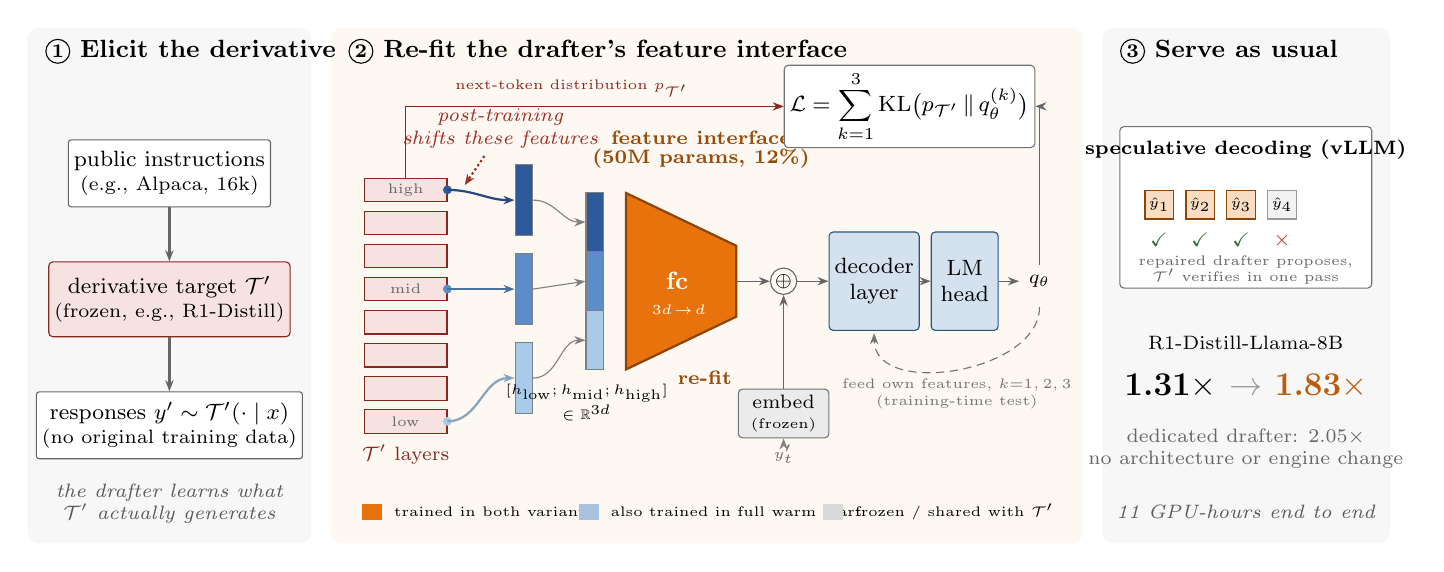
\begin{tikzpicture}[
  font=\footnotesize,
  >={Stealth[length=4pt]},
  doc/.style={draw=black!60, fill=white, rounded corners=1pt, minimum width=2.5cm, minimum height=0.85cm, align=center, inner sep=2pt},
  blk/.style={draw=black!55, rounded corners=1.5pt, align=center, inner sep=2pt},
  layer/.style={draw=derivative!70!black, fill=derivative!14, minimum width=1.05cm, minimum height=0.30cm, inner sep=0pt},
  hdr/.style={font=\small\bfseries, anchor=west},
  feat/.style={draw=black!50, minimum width=0.22cm, minimum height=0.9cm, inner sep=0pt},
  note/.style={font=\scriptsize\itshape, text=black!65, align=center},
]
% ===================== panel backgrounds =====================
\fill[black!3, rounded corners=4pt] (-0.25,-1.55) rectangle (3.35,5.0);
\fill[interface!5, rounded corners=4pt] (3.6,-1.55) rectangle (13.15,5.0);
\fill[black!3, rounded corners=4pt] (13.4,-1.55) rectangle (17.05,5.0);
\node[hdr] at (-0.15,4.7) {\circled{1} Elicit the derivative};
\node[hdr] at (3.7,4.7) {\circled{2} Re-fit the drafter's feature interface};
\node[hdr] at (13.5,4.7) {\circled{3} Serve as usual};

% ===================== (1) elicit =====================
\node[doc] (prompts) at (1.55,3.15) {public instructions\\[-1pt]\scriptsize(e.g., Alpaca, 16k)};
\node[blk, fill=derivative!14, draw=derivative!70!black, minimum width=2.5cm, minimum height=0.95cm] (tgt) at (1.55,1.55) {derivative target $\mathcal{T}'$\\[-1pt]\scriptsize(frozen, e.g., R1-Distill)};
\node[doc] (resp) at (1.55,-0.05) {responses $y' \sim \mathcal{T}'(\cdot \mid x)$\\[-1pt]\scriptsize(no original training data)};
\draw[->, thick, black!60] (prompts) -- (tgt);
\draw[->, thick, black!60] (tgt) -- (resp);
\node[note] at (1.55,-1.05) {the drafter learns what\\$\mathcal{T}'$ actually generates};

% ===================== (2) re-fit =====================
% target stack
\foreach \i in {0,...,7} {
  \node[layer] (L\i) at (4.55,0.0+0.42*\i) {};
}
\node[font=\scriptsize, text=derivative!70!black] at (4.55,-0.42) {$\mathcal{T}'$ layers};
\node[font=\tiny, text=black!60] at (4.55,0.0) {low};
\node[font=\tiny, text=black!60] at (4.55,1.68) {mid};
\node[font=\tiny, text=black!60] at (4.55,2.94) {high};
% taps
\coordinate (tapL) at (5.08,0.0);
\coordinate (tapM) at (5.08,1.68);
\coordinate (tapH) at (5.08,2.94);
\foreach \t/\c in {tapL/featlow, tapM/featmid, tapH/feathigh} { \fill[\c] (\t) circle (1.6pt); }
% feature vectors
\node[feat, fill=featlow] (fl) at (6.05,0.55) {};
\node[feat, fill=featmid] (fm) at (6.05,1.68) {};
\node[feat, fill=feathigh] (fh) at (6.05,2.81) {};
\draw[->, featlow!80!black, thick] (tapL) to[out=0,in=180] (fl.west);
\draw[->, featmid!80!black, thick] (tapM) -- (fm.west);
\draw[->, feathigh!80!black, thick] (tapH) to[out=0,in=180] (fh.west);
% concat vector
\node[feat, minimum height=0.75cm, fill=featlow]  (c1) at (6.95,1.03) {};
\node[feat, minimum height=0.75cm, fill=featmid]  (c2) at (6.95,1.78) {};
\node[feat, minimum height=0.75cm, fill=feathigh] (c3) at (6.95,2.53) {};
\draw[->, black!50] (fl.east) to[out=0,in=180] (c1.west);
\draw[->, black!50] (fm.east) -- (c2.west);
\draw[->, black!50] (fh.east) to[out=0,in=180] (c3.west);
\node[font=\tiny, align=center, anchor=north] at (6.85,0.6) {$[h_{\text{low}};h_{\text{mid}};h_{\text{high}}]$\\$\in\mathbb{R}^{3d}$};
% shift annotation
\node[note, text=derivative!80!black, anchor=south] at (5.75,3.35) {post-training\\shifts these features};
\draw[->, derivative!80!black, densely dotted, thick] (5.55,3.37) -- (5.3,3.0);
% interface trapezoid
\fill[interface, draw=interface!60!black, thick] (7.35,0.66) -- (8.75,1.33) -- (8.75,2.23) -- (7.35,2.9) -- cycle;
\node[font=\small\bfseries, text=white] at (8.0,1.78) {fc};
\node[font=\tiny, text=white] at (8.02,1.42) {$3d\!\to\!d$};
\node[font=\scriptsize\bfseries, text=interface!65!black, align=center] at (8.3,3.45) {feature interface\\[-1pt]\scriptsize(50M params, 12\%)};
\node[font=\scriptsize, text=interface!65!black, align=center] at (8.35,0.55) {\textbf{re-fit}};
% token embedding
\node[blk, fill=black!8, minimum width=1.15cm, minimum height=0.5cm] (emb) at (9.35,0.1) {\scriptsize embed\\[-2pt]\tiny(frozen)};
\node[circle, draw=black!60, inner sep=0.5pt, font=\scriptsize] (plus) at (9.35,1.78) {$\oplus$};
\draw[->, black!60] (8.75,1.78) -- (plus.west);
\draw[->, black!60] (emb.north) -- (plus.south);
\node[font=\tiny, text=black!60] at (9.35,-0.42) {$y'_{t}$};
\draw[->, black!50] (9.35,-0.3) -- (emb.south);
% decoder + head
\node[blk, fill=decoder!22, draw=decoder!70!black, minimum width=1.05cm, minimum height=1.25cm] (dec) at (10.5,1.78) {decoder\\layer};
\node[blk, fill=decoder!22, draw=decoder!70!black, minimum width=0.85cm, minimum height=1.25cm] (head) at (11.65,1.78) {LM\\head};
\draw[->, black!60] (plus.east) -- (dec.west);
\draw[->, black!60] (dec.east) -- (head.west);
\node[font=\scriptsize] (q) at (12.6,1.78) {$q_\theta$};
\draw[->, black!60] (head.east) -- (q.west);
% TTT loop
\draw[->, black!55, densely dashed] (12.6,1.45) to[out=-90,in=-90, looseness=1.0] node[pos=0.5, below, font=\tiny, align=center] {feed own features, $k{=}1,2,3$\\(training-time test)} (10.5,1.12);
% loss
\node[blk, fill=white, minimum height=0.55cm] (loss) at (10.95,4.0) {$\displaystyle \mathcal{L}=\sum_{k=1}^{3}\mathrm{KL}\big(p_{\mathcal{T}'}\,\|\,q^{(k)}_\theta\big)$};
\draw[->, derivative!70!black] (L7.north) |- node[pos=0.72, above, font=\tiny] {next-token distribution $p_{\mathcal{T}'}$} (loss.west);
\draw[->, black!60] (q.north) |- (loss.east);
% legend
\fill[interface] (4.0,-1.25) rectangle (4.25,-1.05); \node[font=\tiny, anchor=west] at (4.28,-1.15) {trained in both variants};
\fill[decoder!45] (6.75,-1.25) rectangle (7.0,-1.05); \node[font=\tiny, anchor=west] at (7.03,-1.15) {also trained in full warm start};
\fill[black!15] (9.85,-1.25) rectangle (10.1,-1.05); \node[font=\tiny, anchor=west] at (10.13,-1.15) {frozen / shared with $\mathcal{T}'$};

% ===================== (3) serve =====================
\node[blk, fill=white, minimum width=3.2cm, minimum height=2.05cm, anchor=north] (srv) at (15.22,3.75) {};
\node[font=\scriptsize\bfseries, anchor=north] at (15.22,3.7) {speculative decoding (vLLM)};
% draft tokens
\foreach \j/\ok in {0/1,1/1,2/1,3/0} {
  \pgfmathsetmacro{\xx}{14.12+0.52*\j}
  \ifnum\ok=1
    \node[draw=interface!60!black, fill=interface!25, minimum size=0.36cm, inner sep=0pt, font=\tiny] at (\xx,2.75) {$\hat y_{\the\numexpr\j+1\relax}$};
    \node[font=\scriptsize, text=benign!70!black] at (\xx,2.3) {\checkmark};
  \else
    \node[draw=black!40, fill=black!5, minimum size=0.36cm, inner sep=0pt, font=\tiny] at (\xx,2.75) {$\hat y_{\the\numexpr\j+1\relax}$};
    \node[font=\scriptsize, text=severe] at (\xx,2.3) {$\times$};
  \fi
}
\node[font=\tiny, text=black!60, align=center] at (15.22,1.92) {repaired drafter proposes,\\$\mathcal{T}'$ verifies in one pass};
\node[font=\scriptsize, align=center] at (15.22,1.0) {R1-Distill-Llama-8B};
\node[font=\large\bfseries, align=center] at (15.22,0.45) {1.31$\times$ \textcolor{black!40}{$\rightarrow$} \textcolor{interface!80!black}{1.83$\times$}};
\node[font=\scriptsize, text=black!60, align=center] at (15.22,-0.35) {dedicated drafter: 2.05$\times$\\no architecture or engine change};
\node[note] at (15.22,-1.15) {11 GPU-hours end to end};
\end{tikzpicture}
}
  \caption{\textbf{\refit{}.} \circled{1} The derivative target $\Tp$ answers public instructions, producing data that reflect what it actually generates; none of its training data, nor the drafter's, is needed. \circled{2} A teacher-forced pass of $\Tp$ exposes the multi-layer hidden states that the drafter reads and the next-token distribution it must match. Post-training has shifted both, so we re-fit the drafter's feature interface (orange, \refitI{}) with its native training-time-test objective, optionally warm-starting the decoder layer and head as well (blue, \refitF{}). \circled{3} The repaired drafter keeps its architecture and format, so it is served with an unchanged engine.}
  \label{fig:method}
\end{figure*}

Given a derivative $\Tp$ and the family drafter $D_{\theta_0}$ of its parent, \refit{} produces a drafter $D_{\theta}$ matched to $\Tp$ without the data used to train either model.
The recipe has three steps (Figure~\ref{fig:method}).

\paragraph{Eliciting the derivative.}
The drafter must predict what $\Tp$ will generate, so we let $\Tp$ show it.
We sample instructions $x$ from a public instruction corpus.
We use 16k instructions from Alpaca \citep{taori2023alpaca}, deduplicated against all evaluation prompts; instructions elicited from the derivative itself, which avoid any external dataset and its license, give the same SPEED-Bench acceptance (Appendix~\ref{app:details}).
We render each instruction with the derivative's chat template and greedily decode a response $y' \sim \Tp(\cdot \mid x)$ of up to 512 tokens.
For a reasoning distill, these responses are long reasoning traces, exactly the text the drafter will face in deployment.
This mirrors sequence-level distillation \citep{kim2016sequence} and drafter alignment \citep{zhou2024distillspec,goel2024direct}, with one difference: only the drafter learns, and only to follow a fixed target.

\paragraph{Re-fitting the drafter.}
For each pair $(x, y')$, a single teacher-forced pass of $\Tp$ provides, at every response position, the three hidden states that enter Eq.~\eqref{eq:interface} and the next-token distribution $p_{\Tp}$.
These two signals address exactly the two shifts identified in \S\ref{sec:census}: the drafter learns to read $\Tp$'s features and to predict $\Tp$'s tokens.
We minimize the drafter's native training-time-test objective (Eq.~\ref{eq:ttt}) with $\tilde p_{\Tp}$ in place of $\tilde p_T$ and $k_{\max} = 3$, starting from the family drafter's parameters $\theta_0$.
We consider two operating points:
\begin{itemize}
  \setlength\itemsep{1pt}
  \item \textbf{\refitF{}}, our default, warm-starts all drafter parameters from $\theta_0$; the token embedding remains shared with $\Tp$.
  \item \textbf{\refitI{}} updates only $W_{\text{fc}}$, 50M parameters or 12\% of the drafter, and leaves the decoder layer and head untouched.
\end{itemize}
Both variants inherit everything the family drafter already knows about drafting and only teach it to read the new target.
This warm start is essential.
The same architecture trained from scratch on the same data and budget falls below even the reused drafter (\S\ref{sec:results}).

\paragraph{Cost and deployment.}
\refit{} takes one pass over 16k examples, or 7.9M response tokens.
Generating the responses and training together take about 11 A40 GPU-hours, of which training the drafter accounts for only 2.2.
\refitI{} trains 13\% faster per step with 12\% less peak memory, and its update is a 100\,MB matrix rather than an 850\,MB drafter.
The repaired drafter has the same architecture, vocabulary and file format as the family drafter, so it is a drop-in replacement in the serving engine.

% =====================================================================
\section{Experimental Setup}
\label{sec:setup}
% =====================================================================

\paragraph{Targets and drafters.}
We study the two reasoning distills from the census: DeepSeek-R1-Distill-Llama-8B, distilled from DeepSeek-R1 into Llama-3.1-8B \citep{deepseek2025r1}, and Llama-3.1-Nemotron-Nano-8B-v1, derived from Llama-3.1-8B-Instruct through distillation and reasoning post-training \citep{bercovich2025nemotron}.
Both share the Llama-3.1 architecture and tokenizer, and hence the family drafters of Llama-3.1-8B-Instruct.
Our main family drafter is the EAGLE-3 drafter that the EAGLE authors released for Llama-3.1-8B-Instruct \citep{li2025eagle3}.
We also repair the production EAGLE-3 drafter distributed with vLLM's speculators library \citep{redhat2025speculators} and the DFlash drafter \citep{chen2026dflash}.
As an upper reference, we use the dedicated EAGLE-3 drafter that the EAGLE authors trained specifically for R1-Distill-Llama-8B.
Nemotron-Nano is served in its default chat mode.
For a second model family, we repair the Qwen3-8B family EAGLE-3 drafter on DeepSeek-R1-0528-Qwen3-8B.

\paragraph{Baselines.}
We compare against
(i) reusing the family drafter unchanged;
(ii) an independent draft model, Llama-3.2-1B-Instruct \citep{llama3herd}, which shares the targets' tokenizer;
(iii) n-gram prompt lookup \citep{saxena2023pld}, a training-free drafter built into vLLM;
(iv) training the same EAGLE-3 architecture from scratch on our repair data with the same budget; and
(v) LoRA adapters on every drafter layer \citep{hu2022lora}, with as many trainable parameters as the interface, on the same data.
All speculative methods propose $K{=}4$ tokens per step.

\paragraph{Benchmarks and metrics.}
We evaluate on SPEED-Bench \citep{abramovich2026speedbench}, a unified benchmark for speculative decoding, using a stratified 128-prompt sample of its qualitative split, which spans eleven domains from coding and math to writing, roleplay and multilingual chat.
For mathematical reasoning, we use MATH-500 \citep{hendrycks2021math,lightman2024verify}, and for long reasoning, MATH problems with responses of up to 8,192 tokens.
Prompts are rendered with each target's default chat template, and responses are generated greedily for up to 512 tokens unless stated otherwise.
We report $p_1$, $\tau$ (including the bonus token) and, for R1-Distill, the \emph{gap closed}, $(\tau_{\text{repair}} - \tau_{\text{reuse}}) / (\tau_{\text{dedicated}} - \tau_{\text{reuse}})$.
We measure end-to-end wall-clock speedup over autoregressive decoding in vLLM on NVIDIA A40 GPUs at batch sizes 1 and 8.
R1-Distill acceptance results average three training seeds; confidence intervals are 95\% paired bootstrap intervals over prompts (and seeds).
Further details are in Appendix~\ref{app:details}.

% =====================================================================
\section{Results}
\label{sec:results}
% =====================================================================

\begin{table*}[t]
  \centering
  \small
  \setlength{\tabcolsep}{3.0pt}
  \begin{tabular}{@{}l c ccccc c ccccc@{}}
    \toprule
    & & \multicolumn{5}{c}{\textbf{R1-Distill-Llama-8B}} & & \multicolumn{5}{c}{\textbf{Nemotron-Nano-8B}} \\
    \cmidrule(lr){3-7} \cmidrule(lr){9-13}
    & Train & $p_1$ (\%) & \multicolumn{2}{c}{$\tau$} & \multicolumn{2}{c}{Speedup} & & $p_1$ (\%) & \multicolumn{2}{c}{$\tau$} & \multicolumn{2}{c}{Speedup} \\
    \cmidrule(lr){3-3} \cmidrule(lr){4-5} \cmidrule(lr){6-7} \cmidrule(lr){9-9} \cmidrule(lr){10-11} \cmidrule(lr){12-13}
    Method & GPU-h & SPEED & SPEED & MATH & bs\,1 & bs\,8 & & SPEED & SPEED & MATH & bs\,1 & bs\,8 \\
    \midrule
    Autoregressive & -- & -- & 1.00 & 1.00 & 1.00$\times$ & 1.00$\times$ & & -- & 1.00 & 1.00 & 1.00$\times$ & 1.00$\times$ \\
    Independent drafter (1B) & -- & 61.3 & 2.44 & 2.97 & 1.26$\times$ & 1.11$\times$ & & 64.7 & 2.65 & 2.79 & 1.37$\times$ & 1.24$\times$ \\
    Family drafter, reused & 0 & 43.0 & 1.76 & 1.93 & 1.31$\times$ & 1.07$\times$ & & 42.9 & 1.76 & 1.69 & 1.29$\times$ & 1.13$\times$ \\
    \midrule
    \textbf{\refitI{} (ours)} & 11 & 62.6 & 2.41 & 2.78 & 1.74$\times$ & 1.27$\times$ & & 61.4 & 2.42 & 2.66 & 1.69$\times$ & 1.39$\times$ \\
    \textbf{\refitF{} (ours)} & 11 & 65.0 & 2.54 & 2.97 & \textbf{1.83$\times$} & \textbf{1.29$\times$} & & 62.9 & 2.49 & 2.86 & \textbf{1.80$\times$} & \textbf{1.42$\times$} \\
    \midrule
    \textcolor{black!60}{Dedicated drafter} & \textcolor{black!60}{1.3k--19k} & \textcolor{black!60}{70.5} & \textcolor{black!60}{2.85} & \textcolor{black!60}{3.84} & \textcolor{black!60}{2.05$\times$} & \textcolor{black!60}{1.41$\times$} & & \multicolumn{5}{c}{\textcolor{black!60}{\emph{not available}}} \\
    \bottomrule
  \end{tabular}
  \caption{\textbf{Main results.} First-token acceptance $p_1$, acceptance length $\tau$ and end-to-end speedup over autoregressive decoding (vLLM, A40, batch sizes 1 and 8). MATH is MATH-500; speedups are measured on SPEED-Bench (MATH-500 speedups in Table~\ref{tab:reasoning}). \refit{} improves every acceptance metric over reuse with 95\% confidence intervals excluding zero, and \refitF{} is the fastest method that does not require a dedicated drafter. Training cost includes generating the repair data; the dedicated drafter's cost is a recipe estimate for 10--40 epochs of the public EAGLE-3 recipe. Batch-size-1 confidence intervals are in Appendix~\ref{app:timing}.}
  \label{tab:main}
\end{table*}

\subsection{Main Results}

Table~\ref{tab:main} summarizes our results.
On R1-Distill-Llama-8B, \refitI{} raises the acceptance length on SPEED-Bench from 1.76 to 2.41 (paired gain $0.650\ci{0.607}{0.692}$) and first-token acceptance from 43.0\% to 62.6\%, closing 59.9\%$\ci{57.6}{62.4}$ of the gap to the dedicated drafter while keeping the decoder fixed.
\refitF{} raises the acceptance length to 2.54 ($0.778\ci{0.731}{0.823}$) and first-token acceptance to 65.0\%, within 5.5 points of the dedicated drafter, closing 71.7\%$\ci{69.2}{74.3}$ of the gap.
The gains are equally strong on mathematical reasoning: on MATH-500, \refit{} raises $\tau$ from 1.93 to 2.78 and 2.97, closing 44\% and 54\% of the gap.
On Nemotron-Nano, where no dedicated drafter exists and repair is the only way to obtain a matched drafter, \refitI{} and \refitF{} raise $\tau$ by $0.655\ci{0.604}{0.707}$ and $0.724\ci{0.662}{0.787}$ on SPEED-Bench, and by 0.98 and 1.17 on MATH-500.
The gains are also broad: both variants improve the acceptance length in all eleven SPEED-Bench domains on both targets, from coding and math to roleplay and multilingual chat (Appendix~\ref{app:domains}).

These gains carry over to wall-clock time.
At batch size 1, \refitI{} and \refitF{} accelerate R1-Distill by 1.74$\times$ and 1.83$\times$, against 1.31$\times$ for the reused drafter and 2.05$\times$ for the dedicated one.
\refitF{} thus delivers 79\% of the dedicated drafter's acceleration over autoregressive decoding for an estimated 0.25\% of its training compute.
On Nemotron-Nano, the speedup rises from 1.29$\times$ to 1.80$\times$.
Measured directly against reuse on the same prompts and server processes, \refitF{} decodes 1.39$\times$ faster on both targets (95\% CI $[1.32, 1.47]$ on R1-Distill and $[1.31, 1.48]$ on Nemotron-Nano).
The improvements persist under batching, where speculative decoding has less idle compute to exploit: at batch size 8, \refit{} lifts the speedup from 1.07$\times$ to 1.29$\times$ on R1-Distill and from 1.13$\times$ to 1.42$\times$ on Nemotron-Nano.

\paragraph{What makes \refit{} work.}
Three ingredients make \refit{} work.
The first is the warm start.
Training the same EAGLE-3 architecture from scratch on the repair data reaches an acceptance length of only 1.52 on SPEED-Bench, below even the unrepaired family drafter and a full token per step below \refitF{}.
A drafter's ability to draft is expensive to acquire, and the family drafter already has it.
The second is supervision from the derivative itself.
Training on the same derivative-generated text, but with the parent's hidden states and next-token distributions as supervision, recovers about 60\% of the gain, because the drafter adapts to the new text.
Supervision from the derivative supplies the rest, a further 0.15 tokens per step for the interface and 0.19 for the entire drafter on SPEED-Bench (0.14 and 0.15 on MATH), with confidence intervals well above zero.
\refit{} needs both the derivative's text and the derivative's signals, which is exactly what eliciting the derivative provides.
The third is a full-parameter update: LoRA adapters on every drafter layer, with as many trainable parameters as the interface, fall short of \refitF{} by 0.09 tokens per step on R1-Distill and 0.06 on Nemotron-Nano at a similar training cost.

\paragraph{\refit{} versus other drafters.}
Training-free n-gram lookup rarely finds long matches in open-ended generation and stays below 1.6 tokens per step on both targets.
The independent Llama-3.2-1B drafter predicts the derivatives well, but it runs sixteen transformer layers per drafted token, and this cost holds it to 1.26$\times$ on R1-Distill and 1.37$\times$ on Nemotron-Nano.
Repaired drafters combine high acceptance with the near-free drafting of a single-layer, target-conditioned head and are the fastest option on both targets and at both batch sizes.

\begin{table}[t]
  \centering
  \small
  \setlength{\tabcolsep}{3.1pt}
  \begin{tabular}{@{}lcccccc@{}}
    \toprule
    & \multicolumn{3}{c}{R1-Distill} & \multicolumn{3}{c}{Nemotron-Nano} \\
    \cmidrule(lr){2-4} \cmidrule(lr){5-7}
    & \multicolumn{2}{c}{MATH-500} & 8k & \multicolumn{2}{c}{MATH-500} & 8k \\
    \cmidrule(lr){2-3} \cmidrule(lr){5-6}
    Method & bs\,1 & bs\,8 & bs\,1 & bs\,1 & bs\,8 & bs\,1 \\
    \midrule
    Reused & 1.48 & 1.33 & 1.33 & 1.33 & 1.36 & 1.12 \\
    Independent (1B) & 1.53 & 1.39 & -- & 1.32 & 1.50 & -- \\
    \refitI{} & 2.14 & 1.93 & 1.63 & \textbf{2.08} & 2.12 & 1.54 \\
    \refitF{} & \textbf{2.31} & \textbf{2.05} & \textbf{1.77} & 1.94 & \textbf{2.23} & \textbf{1.63} \\
    \midrule
    \textcolor{black!60}{Dedicated} & \textcolor{black!60}{2.87} & \textcolor{black!60}{2.54} & \textcolor{black!60}{2.11} & -- & -- & -- \\
    \bottomrule
  \end{tabular}
  \caption{\refit{} on reasoning workloads. Wall-clock speedup ($\times$) over autoregressive decoding on MATH-500 with 512-token responses (batch sizes 1 and 8) and on MATH problems with responses of up to 8,192 tokens (batch size 1). \refit{} is trained on responses of at most 512 tokens.}
  \label{tab:reasoning}
\end{table}

\begin{figure*}[t]
  \centering
  % Figure 3: (a) gap closed vs. repair data; (b) speedup vs. training compute.
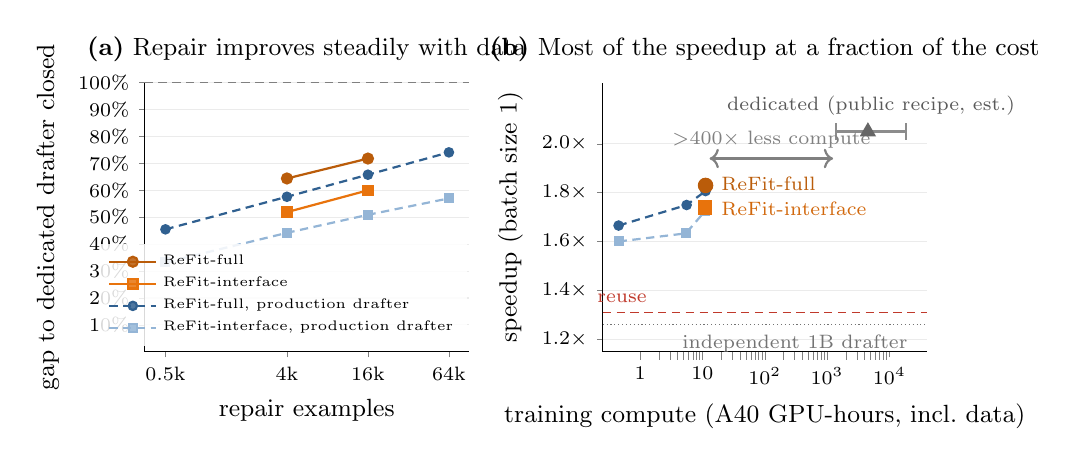
\begin{tikzpicture}
\begin{groupplot}[
  group style={group size=2 by 1, horizontal sep=1.7cm},
  width=0.47\textwidth, height=5.0cm,
  tick label style={font=\scriptsize},
  label style={font=\small},
  title style={font=\small, yshift=-2pt},
  axis x line*=bottom, axis y line*=left,
  tick align=outside, major tick length=2pt,
  grid style={black!8}, ymajorgrids,
  legend style={font=\scriptsize, draw=none, fill=white, fill opacity=0.85, text opacity=1, cells={anchor=west}, row sep=-1pt},
]
% ---------------- (a) data scaling ----------------
\nextgroupplot[
  xmode=log, log basis x=2,
  xmin=0.35, xmax=90,
  xtick={0.5,4,16,64}, xticklabels={0.5k,4k,16k,64k},
  ymin=0, ymax=100,
  ytick={10,20,30,40,50,60,70,80,90,100},
  yticklabel={\pgfmathprintnumber{\tick}\%},
  xlabel={repair examples},
  ylabel={gap to dedicated drafter closed},
  title={\textbf{(a)} Repair improves steadily with data},
  legend style={at={(axis cs:88,2)}, anchor=south east, font=\tiny},
]
\draw[densely dashed, black!50] (axis cs:0.35,100) -- (axis cs:90,100);
\node[font=\scriptsize, black!60, anchor=south east] at (axis cs:88,100) {dedicated drafter};
\addplot[thick, color=interface!80!black, mark=*, mark size=1.8pt] coordinates {(4,64.4) (16,71.8)};
\addlegendentry{ReFit-full}
\addplot[thick, color=interface, mark=square*, mark size=1.7pt] coordinates {(4,51.9) (16,60.0)};
\addlegendentry{ReFit-interface}
\addplot[thick, densely dashed, color=decoder!80!black, mark=*, mark size=1.5pt, mark options={solid}] coordinates {(0.5,45.5) (4,57.6) (16,65.8) (64,74.1)};
\addlegendentry{ReFit-full, production drafter}
\addplot[thick, densely dashed, color=decoder!55, mark=square*, mark size=1.4pt, mark options={solid}] coordinates {(0.5,33.2) (4,44.2) (16,50.9) (64,57.0)};
\addlegendentry{ReFit-interface, production drafter}
% ---------------- (b) cost vs speedup ----------------
\nextgroupplot[
  xmode=log, xmin=0.25, xmax=40000,
  xtick={1,10,100,1000,10000},
  xticklabels={1,10,$10^2$,$10^3$,$10^4$},
  ymin=1.15, ymax=2.25,
  ytick={1.2,1.4,1.6,1.8,2.0},
  yticklabels={1.2$\times$,1.4$\times$,1.6$\times$,1.8$\times$,2.0$\times$},
  xlabel={training compute (A40 GPU-hours, incl.\ data)},
  ylabel={speedup (batch size 1)},
  title={\textbf{(b)} Most of the speedup at a fraction of the cost},
  clip=false,
]
\draw[densely dashed, severe] (axis cs:0.25,1.31) -- (axis cs:40000,1.31) node[pos=0.06, above, font=\scriptsize] {reuse};
\draw[densely dotted, black!55] (axis cs:0.25,1.26) -- (axis cs:40000,1.26) node[pos=0.97, below, font=\scriptsize, anchor=north east] {independent 1B drafter};
% production repairs at three budgets
\addplot[thick, densely dashed, color=decoder!80!black, mark=*, mark size=1.5pt, mark options={solid}] coordinates {(0.45,1.666) (5.56,1.750) (11.2,1.807)};
\addplot[thick, densely dashed, color=decoder!55, mark=square*, mark size=1.4pt, mark options={solid}] coordinates {(0.45,1.601) (5.40,1.634) (10.9,1.724)};
% official repairs (main setting)
\addplot[only marks, color=interface!80!black, mark=*, mark size=2.6pt] coordinates {(11.2,1.83)};
\addplot[only marks, color=interface, mark=square*, mark size=2.4pt] coordinates {(10.9,1.74)};
\node[font=\scriptsize, interface!80!black, anchor=west] at (axis cs:14,1.835) {ReFit-full};
\node[font=\scriptsize, interface!90!black, anchor=west] at (axis cs:14,1.735) {ReFit-interface};
% dedicated drafter: public recipe estimate (10--40 epochs)
\draw[|-|, thick, black!45] (axis cs:1348,2.05) -- (axis cs:19232,2.05);
\addplot[only marks, mark=triangle*, mark size=3pt, color=black!60] coordinates {(4520,2.05)};
\node[font=\scriptsize, black!65, anchor=south] at (axis cs:5100,2.075) {dedicated (public recipe, est.)};
\draw[<->, thick, black!50] (axis cs:13,1.94) -- (axis cs:1250,1.94) node[midway, above, font=\scriptsize] {$>$400$\times$ less compute};
\end{groupplot}
\end{tikzpicture}

  \caption{\textbf{(a)} Gap to the dedicated drafter closed on R1-Distill-Llama-8B as a function of the number of repair examples, for the EAGLE authors' family drafter (solid) and the production drafter (dashed). \textbf{(b)} Batch-size-1 speedup against training compute, including data generation. \refit{} attains most of the dedicated drafter's speedup with orders of magnitude less compute; the dedicated drafter's range spans 10 to 40 epochs of the public recipe.}
  \label{fig:scaling}
\end{figure*}

\subsection{Reasoning Workloads}

Reasoning models are deployed on mathematical and scientific problems, with long generation budgets and often with sampling, whereas \refit{} sees responses of at most 512 tokens.
Table~\ref{tab:reasoning} shows that its absolute speedups are largest exactly there.
On MATH-500, \refitF{} accelerates R1-Distill by 2.31$\times$ at batch size 1 and 2.05$\times$ at batch size 8, compared with 1.48$\times$ and 1.33$\times$ for the reused drafter, and Nemotron-Nano by up to 2.23$\times$.
With responses of up to 8,192 tokens, 2.4k--3.3k on average, \refitF{} still delivers 1.77$\times$ and 1.63$\times$, against 1.33$\times$ and 1.12$\times$ for reuse.
Its gains also hold under temperature sampling ($T{=}0.6$), where verification accepts tokens stochastically: on these long traces, \refitF{} raises the acceptance length from 1.96 to 2.58 on R1-Distill and from 1.64 to 2.63 on Nemotron-Nano (Appendix~\ref{app:long}).

\subsection{Scaling and Cost}

Figure~\ref{fig:scaling}a shows that \refit{} improves steadily with data.
With the production drafter, the gap closed by \refitF{} grows from 46\% with 0.5k examples to 58\% with 4k, 66\% with 16k and 74\% with 64k.
The curve is still rising at 64k examples, and the EAGLE authors' family drafter stays ahead at every budget (64\% at 4k, 72\% at 16k).
\refitI{} follows a parallel curve 12--15 points lower and thus captures most of the benefit of the full warm start with an eighth of the trainable parameters.

Figure~\ref{fig:scaling}b places these results in terms of compute.
Even 0.45 GPU-hours of repair on 256 examples already yield a 1.67$\times$ speedup, and 11 GPU-hours reach 1.83$\times$.
By contrast, we estimate that reproducing the dedicated drafter with the public EAGLE-3 recipe requires between 1.3k and 19k A40 GPU-hours including data generation, depending on the number of epochs.
\refit{} thus recovers most of the dedicated drafter's speedup for 120 to 1,700 times less compute.

\begin{table}[t]
  \centering
  \small
  \setlength{\tabcolsep}{3.4pt}
  \begin{tabular}{@{}llccc@{}}
    \toprule
    & & & \multicolumn{2}{c}{\refit{}} \\
    \cmidrule(l){4-5}
    Family drafter & Target & Reuse & interface & full \\
    \midrule
    \multirow{2}{*}{EAGLE-3 (authors)} & R1 & 1.76 & 2.41 & \textbf{2.54} \\
                                 & Nemotron & 1.76 & 2.42 & \textbf{2.49} \\
    \multirow{2}{*}{EAGLE-3 (production)} & R1 & 1.73 & 2.30 & \textbf{2.47} \\
                                 & Nemotron & 1.82 & 2.32 & \textbf{2.42} \\
    \multirow{2}{*}{DFlash (256 ex.)} & R1 & 2.08 & 2.22 & \textbf{2.31} \\
                                 & Nemotron & 2.08 & 2.24 & \textbf{2.36} \\
    \midrule
    EAGLE-3 (Qwen3) & R1-Qwen3 & 1.93 & 2.18 & \textbf{2.30} \\
    \bottomrule
  \end{tabular}
  \caption{\refit{} generalizes across drafter checkpoints and drafter families. Acceptance length on SPEED-Bench with 16k repair examples (DFlash, which drafts ten-token blocks: 256). R1-Qwen3: DeepSeek-R1-0528-Qwen3-8B.}
  \label{tab:robustness}
\end{table}

\subsection{Generality}

Table~\ref{tab:robustness} shows that \refit{} does not depend on a particular drafter.
The production EAGLE-3 drafter distributed with vLLM is repaired almost as well as the EAGLE authors' drafter, closing 66\% and 51\% of the R1-Distill gap.
Repairing DFlash, a parallel block-diffusion drafter with the same kind of feature interface, on only 256 examples raises its acceptance length by 11--13\%.
\refit{} also repairs drafters in a second model family: the Qwen3-8B family drafter, reused on DeepSeek-R1-0528-Qwen3-8B, gains 0.25 and 0.38 tokens per step on SPEED-Bench from \refitI{} and \refitF{} and 0.47 on MATH-500, raising the batch-size-1 speedup from 1.55$\times$ to 1.85$\times$, ahead of an independent Qwen3 draft model (1.52$\times$).
In all seven settings, \refitI{} alone delivers most of \refitF{}'s gain.

% =====================================================================
\section{Related Work}
\label{sec:related}
% =====================================================================

\paragraph{Speculative decoding.}
Speculative decoding \citep{leviathan2023speculative,chen2023accelerating} has been extended with tree verification \citep{miao2024specinfer,chen2024sequoia}, self-speculation \citep{zhang2024draftverify} and model-free drafting \citep{fu2024lookahead,he2024rest,saxena2023pld,oliaro2024suffix}; see \citet{xia2024survey} for a survey.
The strongest drafters condition on the target's hidden states \citep{cai2024medusa,ankner2024hydra,li2024eagle,li2024eagle2,li2025eagle3,eagle31,zhang2025hass,jiang2026hspec,chen2026dflash}; open frameworks make training them possible but not cheap \citep{li2026specforge,redhat2025speculators}, and vocabulary pruning reduces their cost \citep{zhao2025frspec,goel2025vocabtrim}.
We keep such drafters working when their target changes.

\paragraph{Adapting drafters.}
DistillSpec \citep{zhou2024distillspec} distills a draft model from its target, online speculative decoding \citep{liu2024online} keeps updating it on served traffic, and Draft-OPD \citep{lei2026draftopd} trains drafters on their own on-policy proposals.
Other work aligns drafters with chat-tuned targets \citep{goel2024direct} or new domains \citep{hong2025domain}, adapts them efficiently with EDA \citep{lin2026eda}, shares frozen drafts across evolving targets \citep{li2026flexspec}, or evolves them online \citep{ramakrishnan2025omnidraft,zhang2026evospec}.
These approaches re-align the drafter as a whole or change its architecture or training regime; EDA, for instance, adds gated shared and private experts.
\refit{} keeps the released architecture, so the repaired drafter loads in unchanged engines, and works offline from public instructions, without traffic logs or original training data.

\paragraph{Post-training and representation drift.}
Fine-tuning distorts pretrained features \citep{kumar2022finetuning}, and the extent depends on the training signal: on-policy RL forgets less than supervised training on fixed data \citep{shenfeld2026razor,chen2026retaining}.
Our census connects these findings to inference efficiency in an ecosystem of derivatives \citep{horwitz2025atlas}: the regimes that move a model furthest from its initialization are the ones that break the drafters built for it.

% =====================================================================
\section{Conclusion}
% =====================================================================

Family drafters make speculative decoding practical across the open-model ecosystem, but they silently lose much of their value on the extensively post-trained derivatives that dominate reasoning workloads.
We showed that post-training shifts both the features a drafter reads and the tokens it must predict, and that re-fitting the drafter on the derivative's own responses to public instructions, or even only its feature interface, restores most of a dedicated drafter's speedup for a few GPU-hours.
\refit{} turns per-derivative drafting into a routine step that can accompany every model release: when the target moves, the drafter can learn to follow it from the target itself.

% =====================================================================
\section*{Limitations}
% =====================================================================

Our study focuses on 8B-scale derivatives of the Llama-3.1 and Qwen3 families and on the EAGLE-3 and DFlash drafters, which are among the most widely deployed configurations.
\refit{} requires running the derivative to generate responses; this cost is small and is included in all our compute figures.
We measure wall-clock speedups on NVIDIA A40 GPUs in vLLM with chain drafting, the configuration supported by our serving engine; absolute speedups vary with hardware, batch size and decoding configuration.

\section*{Ethical Considerations}

\refit{} leaves the target model's weights and outputs unchanged: speculative decoding is lossless, so repair affects only serving cost, not what the model generates.
By reducing the compute needed to serve reasoning models, it lowers the energy cost of deploying them.
All models and prompt sources are public and used under their licenses, and no private user data is involved.

\bibliography{custom}

\appendix

% =====================================================================
\section{Implementation Details}
\label{app:details}
% =====================================================================

\paragraph{Repair.}
We optimize Eq.~\eqref{eq:ttt} with AdamW (learning rate $2\times10^{-5}$, weight decay 0.01, cosine schedule with 3\% warm-up) for one epoch over the 16k repair examples, packing roughly 2k response tokens per step, with $k_{\max}{=}3$ training-time-test steps.
The loss is computed on response positions only.
The target's logits are restricted to the 32k draft vocabulary and renormalized before the KL divergence; at successive training-time-test steps the drafter consumes its own predicted features together with the observed response tokens.
Repair data are generated greedily with vLLM, capped at 512 response tokens, and deduplicated exactly and approximately against all evaluation prompts, including the full MATH-500 set.
\refitI{} updates $W_{\text{fc}} \in \mathbb{R}^{4096 \times 12288}$ (50.3M parameters); \refitF{} updates the interface, the decoder layer and the language-modeling head (424.8M parameters), keeping the token embedding shared with the target.
When a released drafter omits the embedding table, the trainer loads the target's embedding, exactly as the serving engine does.
The three R1-Distill seeds use the same data and differ only in the training seed.
Repair costs 11.1 A40 GPU-hours on R1-Distill (8.9 for generating responses, 2.2 for training) and 9.8--10.0 on Nemotron-Nano.

\paragraph{Training resources.}
Over the same 200 training batches, \refitI{} takes 1.57\,s per step at 25.7\,GiB peak memory, against 1.77\,s and 29.1\,GiB for \refitF{}.
Its mutable state is the interface alone: 100.7\,MB in bf16, against 849.4\,MB for the full drafter.
The decoder layer and head of an interface-repaired drafter are bit-identical to the released family drafter.

\paragraph{Instruction source.}
Replacing Alpaca with 4k instructions elicited from the derivative itself, which requires no external dataset, leaves SPEED-Bench acceptance unchanged ($\Delta\tau = 0.004$ and $0.009$ for \refitI{} and \refitF{}, both within noise).

\paragraph{Draft vocabulary.}
\refit{} keeps the family drafter's 32k draft vocabulary.
Re-selecting the vocabulary from the derivative's responses before \refitF{} leaves acceptance unchanged on Nemotron-Nano ($\tau$ 2.47 versus 2.49 on SPEED-Bench, 2.85 versus 2.86 on MATH-500), so the inherited vocabulary is not a bottleneck.

\begin{figure}[h]
  \centering
  % Figure: where to repair -- gap closed vs. trainable parameters, by update location
% (R1-Distill, production EAGLE-3 drafter, 256 repair examples, 300 steps, same recipe; SPEED-Bench).
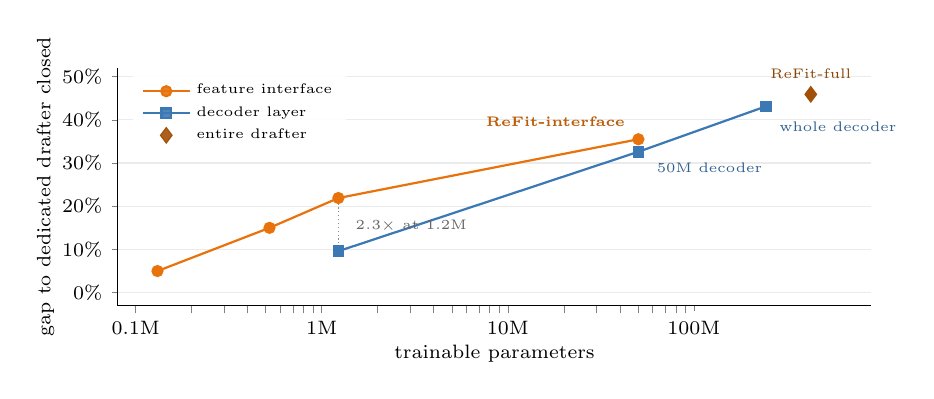
\begin{tikzpicture}
\begin{axis}[
  width=0.92\columnwidth, height=4.6cm,
  xmode=log, xmin=0.08, xmax=900,
  ymin=-3, ymax=52,
  xtick={0.1,1,10,100},
  xticklabels={0.1M,1M,10M,100M},
  ytick={0,10,20,30,40,50},
  yticklabels={0\%,10\%,20\%,30\%,40\%,50\%},
  tick label style={font=\scriptsize},
  xlabel={\scriptsize trainable parameters},
  ylabel={\scriptsize gap to dedicated drafter closed},
  xlabel style={yshift=3pt}, ylabel style={yshift=-4pt},
  axis x line*=bottom, axis y line*=left,
  tick align=outside, major tick length=2pt,
  ymajorgrids, grid style={black!8},
  legend style={font=\tiny, draw=none, fill=white, fill opacity=0.9, text opacity=1, at={(0.02,0.98)}, anchor=north west, cells={anchor=west}, row sep=-1pt},
  clip=false,
]
% interface location
\addplot[thick, color=interface, mark=*, mark size=1.8pt] coordinates {(0.131,5.0) (0.524,15.0) (1.229,21.9) (50.33,35.5)};
\addlegendentry{feature interface}
% decoder location
\addplot[thick, color=decoder, mark=square*, mark size=1.7pt] coordinates {(1.229,9.6) (50.30,32.6) (243.3,43.1)};
\addlegendentry{decoder layer}
% whole drafter
\addplot[only marks, color=interface!70!black, mark=diamond*, mark size=2.8pt] coordinates {(424.8,45.9)};
\addlegendentry{entire drafter}
% equal-capacity guides
\draw[densely dotted, black!45] (axis cs:1.229,9.6) -- (axis cs:1.229,21.9);
\draw[densely dotted, black!45] (axis cs:50.33,32.6) -- (axis cs:50.33,35.5);
\node[font=\tiny, anchor=west, text=black!60] at (axis cs:1.35,15.5) {$2.3\times$ at 1.2M};
% labels
\node[font=\tiny, anchor=south east, text=interface!80!black] at (axis cs:48,36.3) {\textbf{\refitI{}}};
\node[font=\tiny, anchor=north west, text=decoder!80!black] at (axis cs:56,32.3) {50M decoder};
\node[font=\tiny, anchor=south, text=interface!60!black] at (axis cs:424.8,47.2) {\refitF{}};
\node[font=\tiny, anchor=north west, text=decoder!80!black] at (axis cs:255,41.8) {whole decoder};
\end{axis}
\end{tikzpicture}

  \caption{\textbf{Where to repair.} Fraction of the acceptance-length gap between the reused family drafter and a dedicated drafter closed by re-fitting the feature interface or the decoder layer with a given number of trainable parameters (R1-Distill-Llama-8B, production drafter, SPEED-Bench; same 256 repair examples and training recipe for every point). The dense interface (\refitI{}) captures most of what re-training the entire drafter (\refitF{}) achieves, and with little data it outperforms decoder updates of equal size.}
  \label{fig:components}
\end{figure}

\paragraph{Component analysis.}
For Figure~\ref{fig:components}, all variants use the same 256 R1-Distill responses, batches, learning rate and 300 optimization steps, starting from the production EAGLE-3 drafter.
Interface variants are LoRA updates of $W_{\text{fc}}$ with ranks 8, 32 and 75 (0.13M, 0.52M and 1,228,800 parameters) and the dense interface (50,331,648).
Decoder variants are LoRA on the query, value and MLP projections with rank 16 (1,228,800 parameters, exactly matching the rank-75 interface) and rank 655 (50.30M), a full-rank update of the query and output projections (50,331,648, exactly matching the dense interface), and the whole decoder layer (243.3M); the interface and head stay frozen in all decoder variants.
The feature-statistics baseline fits a per-layer affine map that matches the mean and scale of the derivative's tapped features to the parent's.
The parent-supervision control keeps the derivative-generated token sequences, masks, batches, initialization and objective fixed and replaces only the model that supplies the hidden states and next-token distributions.
The whole-drafter LoRA baseline adapts every drafter linear layer (interface, attention, MLP and head) with rank 343 (50.31M parameters) on the 16k repair data.

\paragraph{Crossover.}
For each model, we take 64 contexts generated by the parent, by the derivative, and from public reference text, run both the parent and the derivative on the identical text, and feed each model's tapped hidden states to the frozen family drafter.
Agreement is the rate at which the drafter's first prediction matches a given model's greedy next token.
The feature effect averages the change in agreement from swapping parent features for derivative features under each fixed verifier; the policy effect averages the change from swapping the verifier under each fixed feature source.

\paragraph{Training-time-test depth.}
The drafter is unrolled for $k_{\max}{=}3$ steps during training and proposes $K{=}4$ tokens at serving time.
Training with $k_{\max}{=}4$ instead gives the same acceptance ($\Delta\tau = -0.004$ and $-0.007$ on SPEED-Bench for \refitI{} and \refitF{} at 4k examples, both within noise).

\paragraph{Evaluation.}
All acceptance measurements use vLLM with greedy decoding, $K{=}4$ draft tokens (DFlash: its native block of ten), a maximum of 512 new tokens and batch size 8.
Nemotron-Nano is used with its default chat template, which carries no reasoning-mode instruction.
Prompts that produce no speculative step are excluded pairwise across compared methods.
Speedups are measured on 32 prompts at batch size 1 and 128 at batch size 8, each in three fresh server processes with three warm repetitions, relative to autoregressive decoding of the same prompts; confidence intervals resample processes and prompt batches jointly.
The dedicated drafter's cost is a recipe estimate: the public EAGLE-3 recipe trains on 532k--646k examples, and our measured A40 throughput for generation and training projects 1.3k--19k GPU-hours at 10 to 40 epochs; the cost of the released dedicated checkpoint itself is not reported.

% =====================================================================
\section{Reasoning Workloads}
\label{app:long}
% =====================================================================

The long-reasoning panel uses the first 32 problems of our 64-problem MATH sample, drawn from MATH-500, with response budgets of up to 8,192 tokens; the same engine, prompts and drafters are used as in the main results.
Sampled decoding uses temperature 0.6 and top-$p$ 0.95 with a fixed seed.
No response in any arm exceeds 50\% repeated 4-gram coverage.
Table~\ref{tab:long} reports acceptance lengths.

\begin{table}[h]
  \centering
  \small
  \setlength{\tabcolsep}{4pt}
  \begin{tabular}{@{}llcccc@{}}
    \toprule
    & & & \multicolumn{2}{c}{\refit{}} & \\
    \cmidrule(lr){4-5}
    Target & Decoding & Reuse & interface & full & Dedicated \\
    \midrule
    \multirow{2}{*}{R1} & greedy & 1.97 & 2.59 & \textbf{2.68} & 3.78 \\
                        & sampled & 1.96 & 2.49 & \textbf{2.58} & 3.38 \\
    \multirow{2}{*}{Nemotron} & greedy & 1.65 & 2.53 & \textbf{2.73} & -- \\
                              & sampled & 1.64 & 2.42 & \textbf{2.63} & -- \\
    \bottomrule
  \end{tabular}
  \caption{Acceptance length on MATH problems with responses of up to 8,192 tokens (2.4k--3.3k on average), under greedy decoding and temperature sampling. Every gain over reuse has a 95\% confidence interval excluding zero.}
  \label{tab:long}
\end{table}

% =====================================================================
\section{Timing Details}
\label{app:timing}
% =====================================================================

Table~\ref{tab:timing} reports every wall-clock speedup with its 95\% confidence interval, resampling server processes and prompt batches jointly.
Batch-size-1 panels use 32 prompts, so their intervals are wider than those at batch size 8.

\begin{table*}[t]
  \centering
  \small
  \setlength{\tabcolsep}{4pt}
  \begin{tabular}{@{}llccccc@{}}
    \toprule
    & & \multicolumn{2}{c}{SPEED-Bench} & \multicolumn{2}{c}{MATH-500} & MATH, 8k tokens \\
    \cmidrule(lr){3-4} \cmidrule(lr){5-6} \cmidrule(lr){7-7}
    Target & Method & bs\,1 & bs\,8 & bs\,1 & bs\,8 & bs\,1 \\
    \midrule
    R1-Distill & Reused & 1.31\,{\scriptsize[1.23, 1.39]} & 1.07\,{\scriptsize[0.99, 1.17]} & 1.48\,{\scriptsize[1.44, 1.52]} & 1.33\,{\scriptsize[1.30, 1.36]} & 1.33\,{\scriptsize[1.09, 1.64]} \\
     & Independent (1B) & 1.26\,{\scriptsize[1.20, 1.33]} & 1.11\,{\scriptsize[1.09, 1.14]} & 1.52\,{\scriptsize[1.49, 1.57]} & 1.39\,{\scriptsize[1.36, 1.42]} & -- \\
     & \refitI{} & 1.74\,{\scriptsize[1.58, 1.89]} & 1.27\,{\scriptsize[1.10, 1.47]} & 2.14\,{\scriptsize[2.10, 2.19]} & 1.93\,{\scriptsize[1.89, 1.98]} & 1.63\,{\scriptsize[1.29, 2.08]} \\
     & \refitF{} & 1.83\,{\scriptsize[1.65, 1.99]} & 1.29\,{\scriptsize[1.12, 1.50]} & 2.31\,{\scriptsize[2.25, 2.36]} & 2.05\,{\scriptsize[2.01, 2.10]} & 1.77\,{\scriptsize[1.44, 2.27]} \\
     & Dedicated & 2.05\,{\scriptsize[1.85, 2.25]} & 1.41\,{\scriptsize[1.20, 1.67]} & 2.87\,{\scriptsize[2.80, 2.95]} & 2.54\,{\scriptsize[2.43, 2.63]} & 2.11\,{\scriptsize[1.68, 2.75]} \\
    \midrule
    Nemotron-Nano & Reused & 1.29\,{\scriptsize[1.20, 1.38]} & 1.13\,{\scriptsize[1.05, 1.20]} & 1.32\,{\scriptsize[1.29, 1.36]} & 1.36\,{\scriptsize[1.19, 1.69]} & 1.12\,{\scriptsize[1.00, 1.28]} \\
     & Independent (1B) & 1.37\,{\scriptsize[1.28, 1.47]} & 1.24\,{\scriptsize[1.20, 1.27]} & 1.31\,{\scriptsize[1.08, 1.52]} & 1.50\,{\scriptsize[1.29, 1.84]} & -- \\
     & \refitI{} & 1.69\,{\scriptsize[1.48, 1.89]} & 1.39\,{\scriptsize[1.22, 1.60]} & 2.08\,{\scriptsize[2.02, 2.14]} & 2.12\,{\scriptsize[1.82, 2.64]} & 1.54\,{\scriptsize[1.31, 1.86]} \\
     & \refitF{} & 1.80\,{\scriptsize[1.63, 1.98]} & 1.42\,{\scriptsize[1.23, 1.67]} & 1.94\,{\scriptsize[1.58, 2.25]} & 2.23\,{\scriptsize[1.92, 2.75]} & 1.63\,{\scriptsize[1.37, 2.02]} \\
    \bottomrule
  \end{tabular}
  \caption{Wall-clock speedup over autoregressive decoding with 95\% confidence intervals (vLLM, A40; three fresh server processes with three warm repetitions each).}
  \label{tab:timing}
\end{table*}

% =====================================================================
\section{Per-Domain Results}
\label{app:domains}
% =====================================================================

Table~\ref{tab:domains} reports the acceptance length on each of SPEED-Bench's eleven domains (11--12 prompts each).
\refitF{} improves every domain on both targets, including multilingual chat, although the repair data contain only English instructions.

\begin{table}[!h]
  \centering
  \small
  \setlength{\tabcolsep}{3.0pt}
  \begin{tabular}{@{}lccccc@{}}
    \toprule
    & \multicolumn{3}{c}{R1-Distill} & \multicolumn{2}{c}{Nemotron-Nano} \\
    \cmidrule(lr){2-4} \cmidrule(lr){5-6}
    Domain & Reuse & \refitF{} & Ded. & Reuse & \refitF{} \\
    \midrule
    coding & 1.92 & 2.86 & 3.30 & 1.70 & 2.76 \\
    humanities & 1.74 & 2.50 & 2.75 & 1.89 & 2.61 \\
    math & 1.94 & 2.86 & 3.36 & 1.71 & 2.68 \\
    multilingual & 1.51 & 1.84 & 1.93 & 1.54 & 1.73 \\
    QA & 1.66 & 2.53 & 2.81 & 1.68 & 2.44 \\
    RAG & 1.87 & 2.68 & 2.94 & 2.14 & 2.76 \\
    reasoning & 1.80 & 2.77 & 3.09 & 1.80 & 2.83 \\
    roleplay & 1.64 & 2.24 & 2.53 & 1.44 & 1.96 \\
    STEM & 1.75 & 2.67 & 2.93 & 1.78 & 2.64 \\
    summarization & 1.84 & 2.54 & 2.85 & 1.92 & 2.47 \\
    writing & 1.72 & 2.44 & 2.83 & 1.80 & 2.45 \\
    \bottomrule
  \end{tabular}
  \caption{Acceptance length on each SPEED-Bench domain. Every gain over reuse has a 95\% confidence interval excluding zero.}
  \label{tab:domains}
\end{table}

% =====================================================================
\section{Census Details}
\label{app:census}
% =====================================================================

The census covers 174 derivatives, 87 in each of the Llama-3.1-8B and Qwen3-8B families, that load with the architecture and tokenizer of the instruction-tuned parent and its released production EAGLE-3 and DFlash drafters.
Post-training histories are taken from model cards; models whose cards describe several stages are grouped by their combined history.
For 163 derivatives, retention is computed on 64 prompts from the derivative's own domain (Table~\ref{tab:census}); the remaining 11 use 128 general prompts.
The reasoning distills and the controls discussed in \S\ref{sec:census} are evaluated on 128 SPEED-Bench prompts.
Group means weight checkpoints equally, with hierarchical bootstrap intervals over checkpoints and paired prompts; per-model results will be released with the paper.
The compatibility probe ranks derivatives by acceptance retention on 16 fixed requests; its AUROC for identifying derivatives whose retention on the remaining, disjoint requests falls below 90\% is 0.91 for EAGLE-3 (14 of 163 degraded) and 0.93 for DFlash (17 of 163), and 1.00 and 0.95 on a separate 21-checkpoint SPEED-Bench cohort.

\begin{table}[h]
  \centering
  \scriptsize
  \setlength{\tabcolsep}{2.0pt}
  \begin{tabular}{@{}lcccccc@{}}
    \toprule
    & \multicolumn{3}{c}{Llama-3.1-8B} & \multicolumn{3}{c}{Qwen3-8B} \\
    \cmidrule(lr){2-4} \cmidrule(lr){5-7}
    History & $n$ & EAGLE-3 & DFlash & $n$ & EAGLE-3 & DFlash \\
    \midrule
    quantization & 11 & 1.00 & 0.99 & 23 & 1.00 & 1.00 \\
    repack & 2 & 1.00 & 0.98 & -- & -- & -- \\
    merge & 3 & 0.98 & 0.96 & 1 & 1.05 & 1.00 \\
    CPT + merge & -- & -- & -- & 1 & 0.93 & 1.03 \\
    SFT + merge & -- & -- & -- & 1 & 1.08 & 1.01 \\
    preference + merge & -- & -- & -- & 1 & 0.95 & 0.94 \\
    abliteration & 22 & 0.98 & 0.96 & 8 & 1.03 & 1.02 \\
    adversarial training & 1 & 1.03 & 0.95 & -- & -- & -- \\
    on-policy RL & -- & -- & -- & 4 & 1.01 & 0.98 \\
    SFT + on-policy RL & 1 & 0.99 & 0.99 & 3 & 1.04 & 1.00 \\
    expert iteration + RL & -- & -- & -- & 1 & 1.24 & 1.03 \\
    preference opt. & 9 & 0.95 & 0.95 & 1 & 0.96 & 0.96 \\
    SFT + preference & 3 & 0.98 & 0.89 & 2 & 1.03 & 0.91 \\
    SFT & 5 & 0.93 & 0.82 & 10 & 1.14 & 1.06 \\
    self-distillation & -- & -- & -- & 1 & 1.01 & 0.99 \\
    teacher distillation & 2 & 0.83 & 0.83 & -- & -- & -- \\
    SFT + teacher distill. & 1 & 1.27 & 1.29 & 1 & 1.07 & 1.08 \\
    teacher distill. + SFT & -- & -- & -- & 2 & 1.09 & 1.04 \\
    SFT + distill. + pref. & 1 & 0.87 & 0.86 & -- & -- & -- \\
    distillation (unspecified) & -- & -- & -- & 1 & 2.21 & 1.67 \\
    undocumented & 25 & 1.00 & 0.96 & 16 & 1.03 & 1.01 \\
    \bottomrule
  \end{tabular}
  \caption{First-token acceptance retention by family and post-training history on each derivative's own-domain prompts.}
  \label{tab:census}
\end{table}

\end{document}
